\textit{}\chapter{永磁同步电机矢量控制}\label{ch:FOC}
\section{引言}
矢量控制可分为直接转矩控制(DTC)和磁场定向控制(FOC),直接转矩控制是通过控制定子电压从而改变定子磁通与转子磁通夹来实现转矩控制,该方法不需要坐标变换,不直接控制电流,结构简单,动态性能高。磁场定向控制是基于解耦的dq轴电流控制,d轴控制磁通,q轴控制电磁转矩,该方法需要运用坐标变换,结构比直接转矩控制复杂,但其稳态性能比直接转矩控制好,电流谐波低\cite{del2006comparison,__2008}.本文所涉及的矢量控制是磁场定向控制。本章主要介绍矢量控制基本原理、反电动势解耦、控制器参数设计方法和基于反电动势的转子位置估算方法。

\section{矢量控制基本原理}
根据第\ref{ch:model}章的建模,在dq坐标系下永磁同步电机的电压方程为:
\begin{align}\label{eq:vdqFinal}
v_{d}&=Ri_{d}+L_{d}\frac{d}{dt}i_{d}-\omega_{r}\lambda_{q}\\
v_{q}&=Ri_{q}+L_{q}\frac{d}{dt}i_{q}+\omega_{r}\lambda_{d}\label{eq:vol_q}
\end{align}
磁链方程可以表示为:
\begin{align}
\lambda_{d}&=L_{d}i_{d}+\lambda_{mpm}\label{eq:flux_d}\\
\lambda_{q}&=L_{q}i_{q}
\end{align}
电磁转矩方程为:
\begin{align}
T_{e}=\frac{3}{2}P\left[\lambda_{mpm}i_{q}+(L_{d}-L_{q})i_{d}i_{q}\right]
\end{align}
电磁转矩方程可以分为两个部分,第一个部分为q轴电流和永磁体磁场相互作用产生的转矩,第二部分为转子dq两轴电感不相等,也就是凸极效应带来的转矩,称磁阻转矩。对于表面贴磁的永磁同步电机,$L_{d}=L_{q}$,不存在磁阻转矩,而对于内嵌永磁体型永磁同步电机,因为$L_{d}$$\neq$$L_{q}$, 存在磁阻转矩。
根据永磁同步电机驱动系统的运动平衡方程\ref{eq:mechanical},通过控制电机输出的电磁转矩实现控制电机转速,当电机电磁转矩大于负载转矩时,电机加速,电磁转矩小于负载转矩时电机转速下降。矢量控制一般具有四种控制策略,分别为:
\begin{itemize}
	\item $i_{d}=0$控制
	
该方式控制$i_{d}=0$,该控制方式使得永磁同步电机与他励直流电动机一样,定子电流只存在转矩分量,电机输出电磁转矩与q轴电流成正比,大小为$T_{e}=\frac{3}{2}P\lambda_{mpm}i_{q}$。该控制方法控制比较简单,转矩特性好。但由于没有弱磁电流,电机调速范围受限。
	\item $i_{d}<0$弱磁控制
	
根据q轴电压方程\ref{eq:vol_q}和d轴磁链方程\ref{eq:flux_d}可知,当转速增大时,需要更高的q轴电压。当转速上升超过一定值时,逆变器将不能提供更高的电压,此时必须要降低d轴磁链,即控制$i_{d}<0$,弱磁增速。
	\item 功率因数$\cos{\varphi}=1$
	
功率因数$\cos{\varphi}=1$控制通常是为了最大化利用逆变器容量,此时电压矢量与电流矢量方向一致,电机功率因数等于1,但由于负载变化时,不能调节永磁同步电机转子励磁,使得电枢电流与电磁转矩不再保持线性关系。
	\item 最大转矩/电流控制
	
在输出相同电磁转矩的情况下,减小电机电流能够降低电机绕组铜耗,降低系统成本,提高效率。对于表面贴磁型永磁同步电机,$T_{e}=\frac{3}{2}P\lambda_{mpm}i_{q}$,控制$i_{d}=0$即为最大转矩/电流控制。对于内嵌永磁体永磁同步电机,由于存在磁阻转矩,$i_{d}=0$不再是最大转矩/电流控制方式。此时,需要计算出不同工作状态下$i_{d}$和$i_{q}$特定组合,使得转矩最大而电流最小\cite{mtpa_2011,lee_mtpa_2010}。	
\end{itemize}

本文所述的矢量控制为$i_{d}=0$控制,永磁电机主磁通完全由转子永磁体提供,通过控制$i_{q}$来控制电磁转矩,此时永磁同步电机可等效为他励直流电动机。该方法控制永磁同步电机较为简单。
\subsection{矢量控制框图}
图\ref{fig:focStructure}所示的为永磁同步电机电流转速双闭环矢量控制框图。根据该框图,转速给定与转子转速反馈比较,偏差经过$PI$调节,其输出作为$q$轴电流内环给定,该给定与$q$轴电流反馈比较经过$PI$控制器,输出作为$q$轴电压指令。$d$轴电流给定为0。$dq$轴电压指令通过$dq$到$\alpha\beta$变换,通过空间矢量调制法生成$PWM$信号控制逆变器,实现电机控制。

根据该框图可以看到,电流反馈需要采集电机三相电流,需要用到电流互感器,坐标变换需要电机转子位置,速度反馈时需要用到转子转速,转速和转子位置信息通常通过使用编码器获取,也可采用算法估算,基于反电动势的位置估算方法将在本章后面介绍。
\begin{figure}[H]
	\centering
	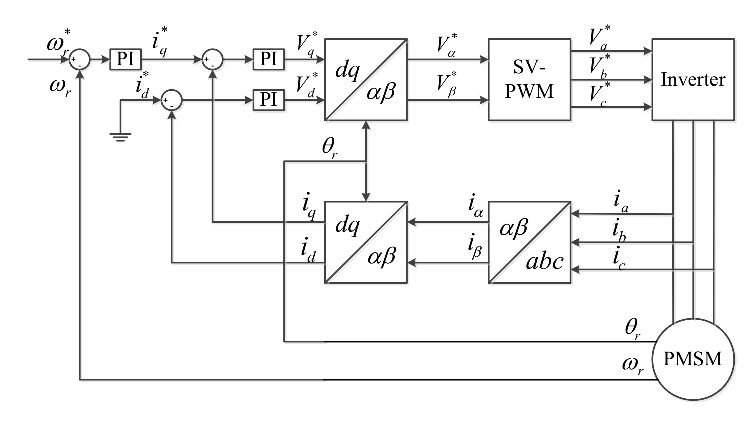
\includegraphics[width=0.7\textwidth]{figs/focStructure.eps}
	\caption{永磁同步电机矢量控制结构框图}
	\label{fig:focStructure}
\end{figure}
\section{矢量控制参数设计调节}
\subsection{基本设计原则}
根据矢量控制框图,可以看到永磁同步电机电流转速双闭环矢量控制中需要用三个PI控制器,两个电流内环PI控制器和一个速度外环PI控制器。调节好这三个PI控制器是实现永磁同步电机矢量控制的关键。双闭环设计原则为:
\begin{itemize}
	\item 先设计电流内环PI控制器,再设计转速外环PI控制器。
	\item 电流内环带宽应为转速外环带宽的10倍左右。
	\item 电流内环不应有超调,如有超调,最大超调不能超过$5\%$。
	\item 转速外环超调应小于$20\%$。
\end{itemize}
\subsection{电流内环PI参数设计}
根据第\ref{ch:model}章建模,可知永磁同步电机d轴电压方程为
\begin{equation}\label{eq:voltage_d}
v_{d}=Ri_{d}+\frac{d}{dt}\lambda_{d}-\omega_{r}L_{q}i_{q}
\end{equation}
采用PI控制器对d轴电流进行反馈控制,控制器给定为d轴电流给定值,输出为d轴电压,控制器传递函数为:
\begin{equation}\label{eq:PI_controller}
	G_{pi}=K_{p}+\frac{K_{i}}{s}
\end{equation}
根据d轴电压方程和PI控制器传递函数可得到d轴PI控制框图\ref{fig:d_PI}所示,可以看到当$\omega_{r}\neq0$时d轴电流调节受到q轴电流和转速的影响,其影响来源于d轴电机模型中的耦合项$\omega_{r}L_{q}i_{q}$,处理该耦合项一般有两种方法,一种将其当作干扰项,也就是图\ref{fig:d_PI}所示的控制结构,其用PI控制器来补偿耦合干扰项,但PI控制器的性能会受到同步参考系角频率的影响,当同步参考系角频率接近控制器带宽时,控制器跟踪给定的性能下降\cite{briz2000analysis},且dq轴并没有实现真正的解耦,例如负载的突变会因为耦合项的存在使得d轴有冲击电流。
\begin{figure}[H]
	\centering
	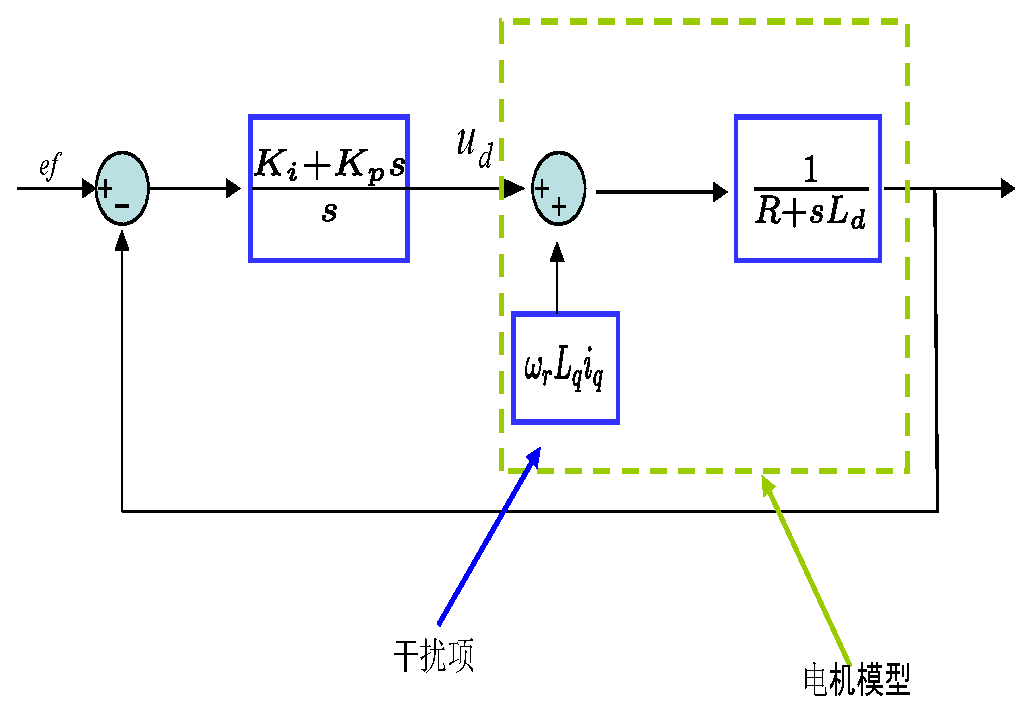
\includegraphics[width=0.7\textwidth]{figs/d_PI.eps}
	\caption{d轴电流环控制框图}
	\label{fig:d_PI}
\end{figure}
另一种方法是按照\ref{fig:d_PI_decoupled}所示的方式对d轴控制器输出电压进行补偿,虽然电机模型不能够改变,但是可以先根据反馈量计算出耦合量,在PI输出端进行补偿。根据该控制框图,PI控制器输出端的补偿项刚好跟电机模型中的耦合项相互抵消,该解耦方法称为反电动势解耦。以上为d轴的解耦方式,q轴可以根据电压方程类似处理。
\begin{figure}[H]
	\centering
	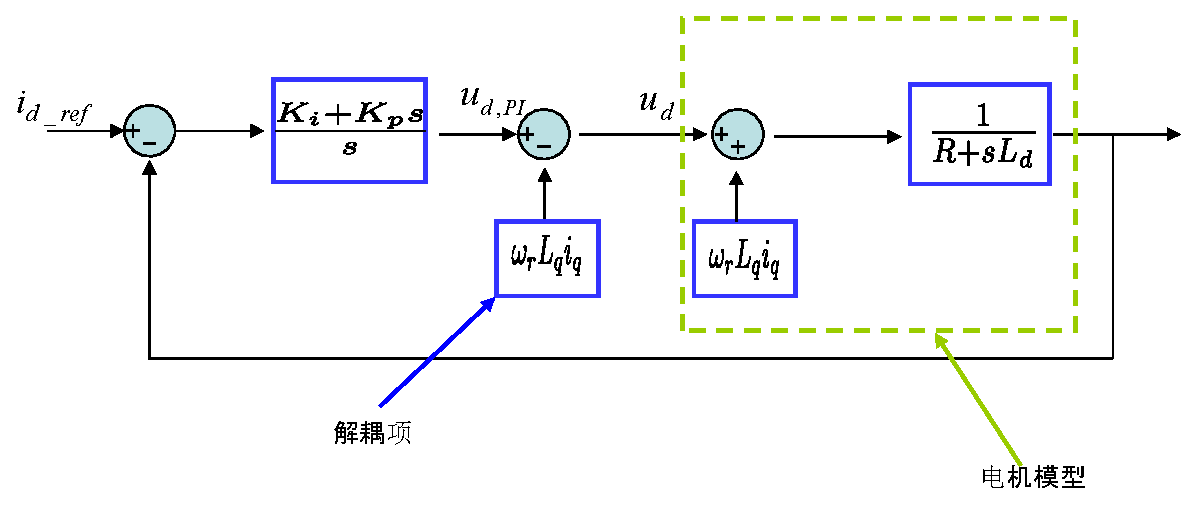
\includegraphics[width=0.7\textwidth]{figs/d_PI_decoupled.eps}
	\caption{解耦的d轴电流环控制框图}
	\label{fig:d_PI_decoupled}
\end{figure}
反电动势解耦之后,d轴电流环控制框图\ref{fig:d_PI_decoupled}可以等效为图\ref{fig:d_PI_decoupled_simple},等效之后电机模型为串联电感电阻,其传递函数为一阶传递函数,结构简单。
\begin{figure}[H]
	\centering
	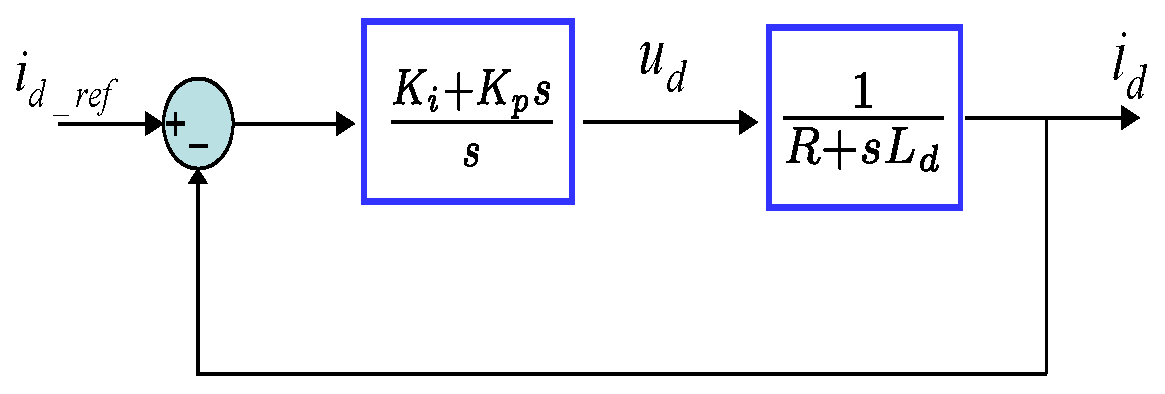
\includegraphics[width=0.7\textwidth]{figs/d_PI_decoupled_simple.eps}
	\caption{简化的解耦的d轴电流环控制框图}
	\label{fig:d_PI_decoupled_simple}
\end{figure}
令PI控制器和电机定子d轴时间常数分别为$\tau_{c}=\frac{K_{p}}{K_{i}}$,$\tau_{e}=\frac{L_{d}}{R}$,图\ref{fig:d_PI_decoupled_simple}可以转化为:
\begin{figure}[H]
	\centering
	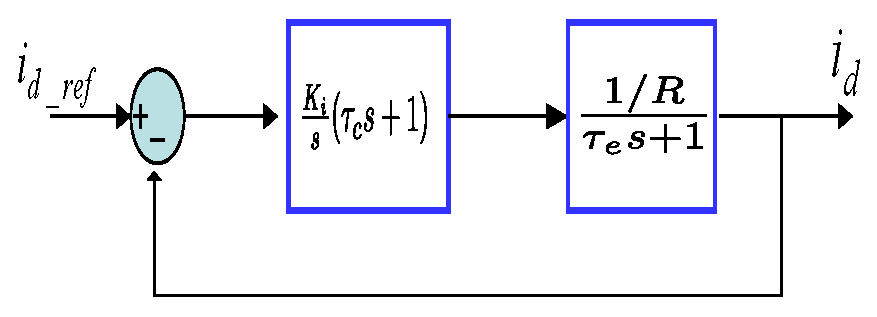
\includegraphics[width=0.7\textwidth]{figs/d_PI_time_const_format.eps}
	\caption{d轴电流内环控制框图}
	\label{fig:d_PI_time_const_format}
\end{figure}
电流环控制框图中,PI控制器提供一个极点一个零点,d轴模型提供一个极点,把控制器零点设置在d轴模型极点上,即$\tau_{c}=\tau_{e}$,这样控制器零点和d轴模型极点形成零极点对消,此时\ref{fig:d_PI_time_const_format}可进一步简化为:
\begin{figure}[H]
	\centering
	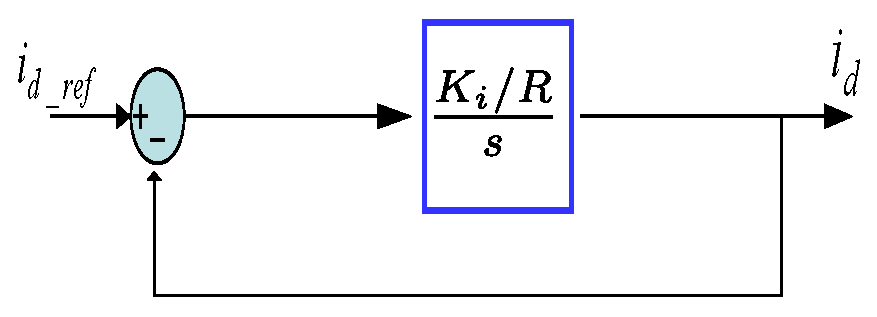
\includegraphics[width=0.7\textwidth]{figs/d_PI_simplest.eps}
	\caption{零极点对消后d轴电流内环}
	\label{fig:d_PI_simplest}
\end{figure}
此时,电流内环开环系统为一个积分和一个比例,其闭环传递函数为:
\begin{equation}
\frac{I_{d}(s)}{I_{d\_ref}(s)}=\frac{K_{i}}{Rs+K_{i}}
\end{equation}
设计电流内环一个重要参数是其带宽,系统带宽的定义为闭环传递函数幅频特性穿越-3dB的频率,系统带宽越高,响应越迅速,但对系统要求也越高\cite{control_theory}。系统闭环传递函数的的幅值随频率变化的表达式为:
\begin{equation}\label{eq:mag_vs_f}
\left|\frac{I_{d}(s)}{I_{d\_ref}(s)}\right|=\frac{K_{i}}{\sqrt{(2 \pi fR)^2+K_{i}^{2}}}
\end{equation}
在-3dB这一点时,式\ref{eq:mag_vs_f}的值为0.707,此时$2\pi f_{bw}R=K_{i}$,$f_{bw}$为带宽频率,根据此等式,可根据所需要的带宽确定电流内环$K_{i}$参数,根据$K_{p}$和$K_{i}$的比例关系即可确定$K_{p}$。参数计算公式\ref{eq:K_i}和\ref{eq:K_p}所示。
\begin{align}
K_{i} &= 2\pi f_{bw} R\label{eq:K_i}\\
K_{p} &= 2\pi f_{bw} L_{d}\label{eq:K_p}
\end{align}

本文仿真所用永磁同步电机参数为$L_{d}=L_{q}=1.7mH$,$R=0.353\Omega$。选择不同带宽,按照公式\ref{eq:K_i}和\ref{eq:K_p}分别选择不同PI控制参数所得的d轴电流阶跃响应如图\ref{fig:current_step}。
\begin{figure}[H]
	\centering
	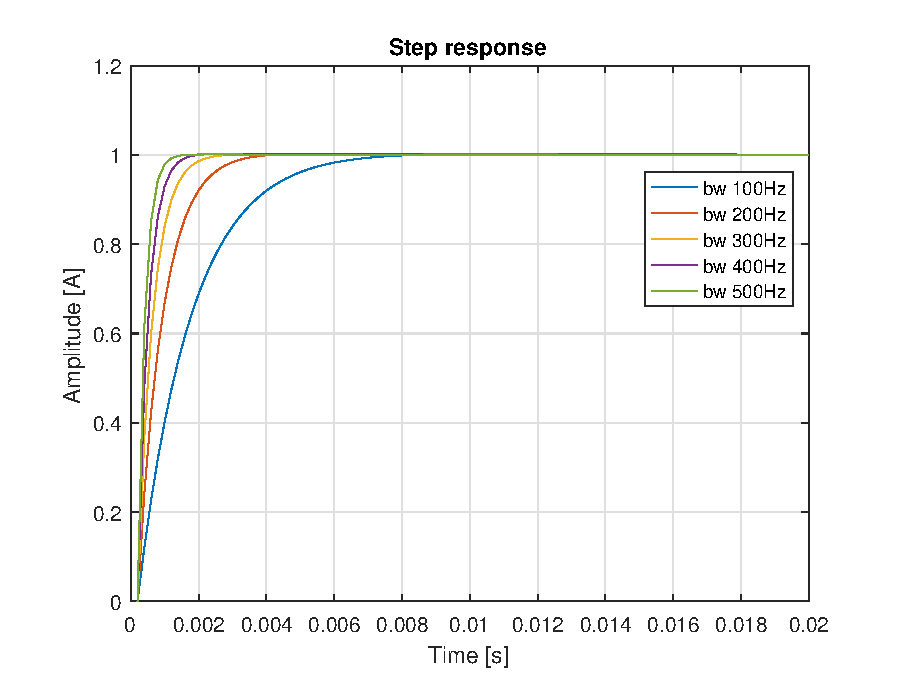
\includegraphics[width=0.7\textwidth]{figs/current_step.eps}
	\caption{不同带宽下的d轴电流阶跃响应}
	\label{fig:current_step}
\end{figure}
以上是d轴电流环参数设计,对于表面贴磁型永磁同步电机,dq两轴参数一致,因此q轴可以选用d轴相同的PI参数。
\subsection{转速外环PI参数调节}
设计好了电流内环之后,调节转速外环PI参数。根据电机运动平衡方程\ref{eq:mechanical},把负载转矩当作干扰项,可得到转矩到转速的传递函数为:
\begin{equation}
	G_{\omega}(s)=\frac{1}{J_{m}s+B_{m}}
\end{equation}
那么不带PI控制器的转速闭环框图如下:
\begin{figure}[H]
	\centering
	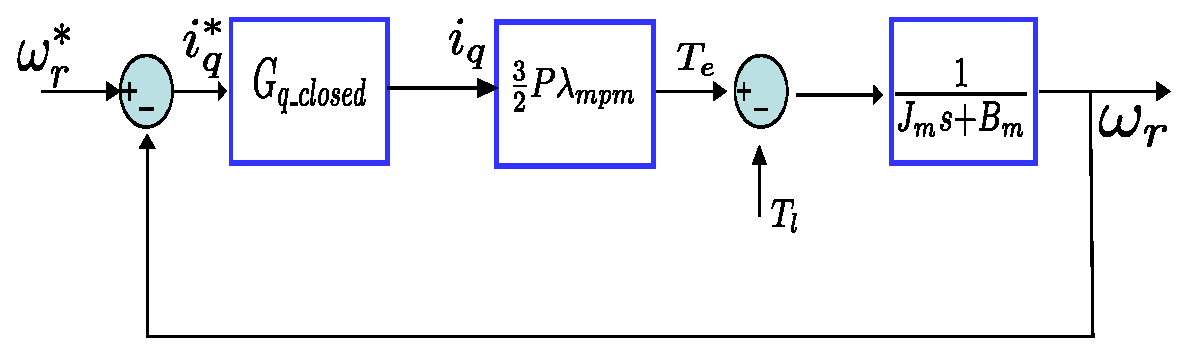
\includegraphics[width=0.7\textwidth]{figs/speed_without_PI.eps}
	\caption{不带PI控制器的转速环框图}
	\label{fig:speed_without_PI}
\end{figure}
其中$G_{q\_closed}$为电流内环。由于摩擦因数$B_{m}$一般很小,转矩到转速的传递函数可以认为是纯积分单元。
\begin{figure} [h]
	\centering%
	\subfloat[空载]{%
		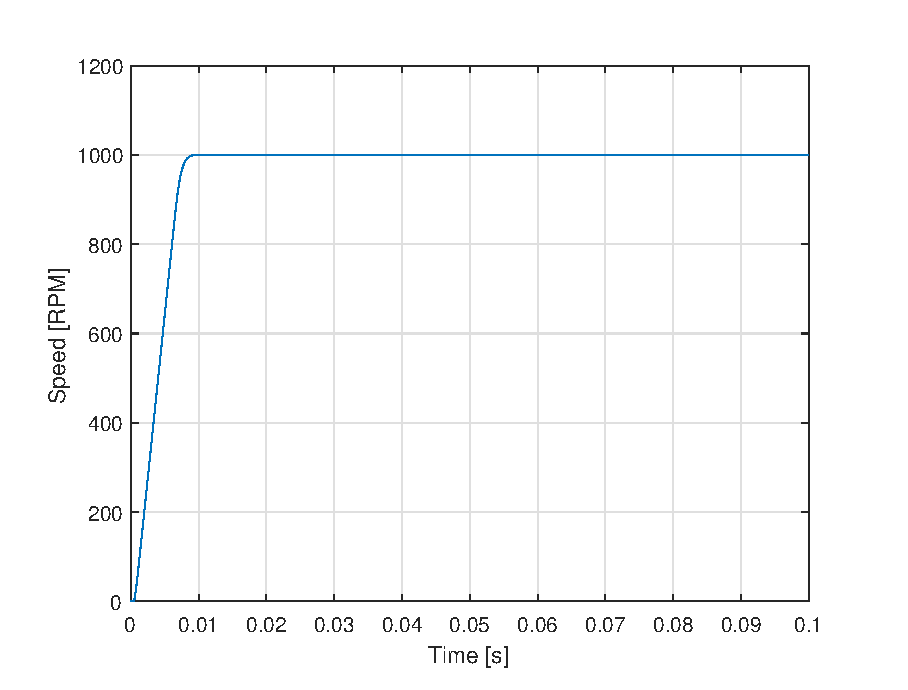
\includegraphics[height=5cm]{figs/kp_speed_no_load.eps}}\hspace{2em}%
	\subfloat[阶跃负载]{%
		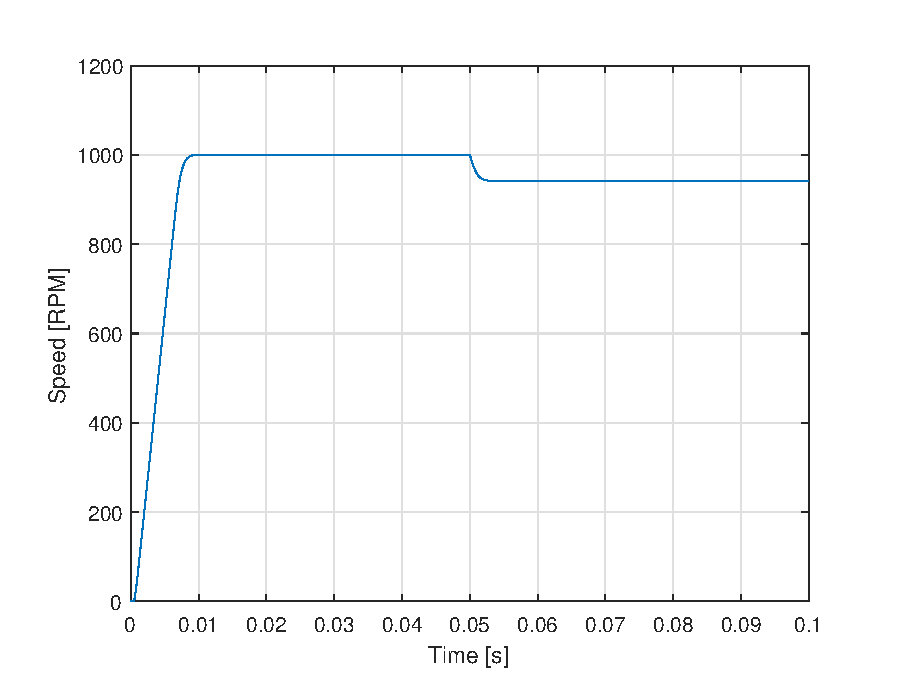
\includegraphics[height=5cm]{figs/kp_speed_step_load.eps}}
	\caption{比例控制转速闭环}
	\label{fig:Kp_speed_loop}
\end{figure}
图\ref{fig:Kp_speed_loop}为比例控制器转速闭环,$K_{p}=0.05$,转速给定值为1000RPM,a为空载运行,b为0.05秒时提供1Nm负载。由该图可知负载转矩$T_{l}=0$时,只用一个比例调节即可实现转速无稳态误差。当存在负载转矩时,只用比例调节系统存在稳态误差,根据公式\ref{eq:steady_state_error}该稳态误差由比例环节参数$K_{p}$和负载转矩$T_{l}$决定,负载越大,稳态误差越大。因此,需要使用PI控制器,来消除带负载时的稳态误差。
\begin{equation}\label{eq:steady_state_error}
e_{ss}=\frac{T_{l}}{K_{p}\frac{3}{2}P\lambda_{mpm}}
\end{equation}
带PI控制器的转速外环控制器框图为:
\begin{figure}[H]
	\centering
	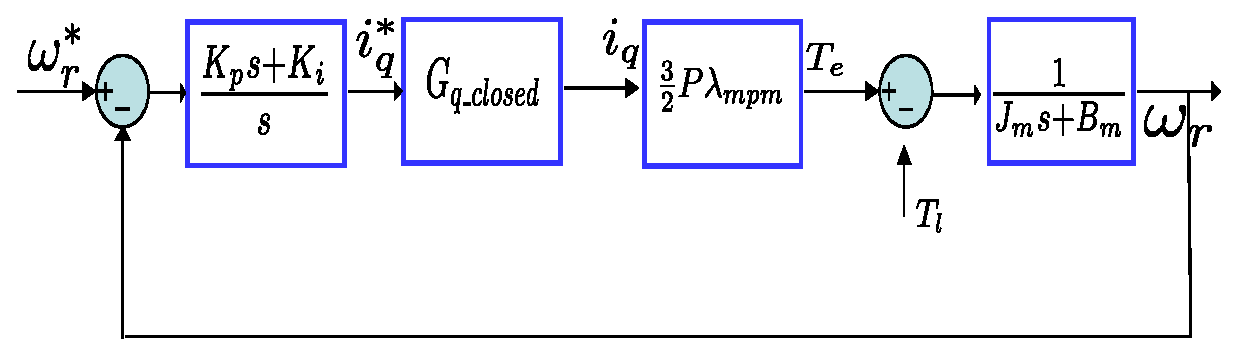
\includegraphics[width=0.7\textwidth]{figs/speed_with_PI.eps}
	\caption{带PI控制器的转速环框图}
	\label{fig:speed_with_PI}
\end{figure}
速度外环参数调节时,先调节$K_{p}$,增大$K_{p}$系统响应快速性达到要求,再调节使其能够快速消除稳态误差。
\subsection{抗饱和PI控制器}
前面讨论电流转速环PI参数时,均忽略了PI控制器输出限制幅值,由于实际变频器输出输出电压范围和电机最大电流有限,因此实际系统中电流内环与转速外环PI控制器输出均有限幅。控制器输出限幅值,使电机在能够保护设备,但当给定转速或者电流很大时,控制器输出饱和,但是实际转速或者电流依然小于给定,因此控制器将长时间在饱和区,这增加了系统超调,甚至可能会引起系统不稳定。
为了解决这一问题,采用抗饱和PI控制器。其框图如图\ref{fig:antiwindup_pi}所示,输出不饱和时和传统PI控制器一样,当输出饱和时,积分器的作用会使系统更快速退出饱和状态,减小超调\cite{antiwindup,antiwindup1,anti_windup_2}。
\begin{figure}[H]
	\centering
	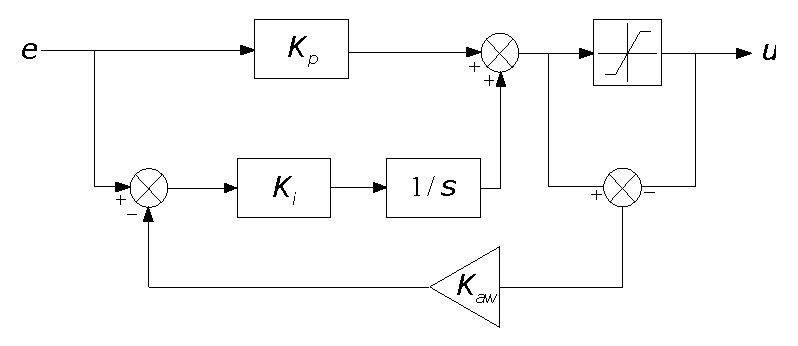
\includegraphics[width=0.7\textwidth]{figs/antiwindup_pi.eps}
	\caption{抗饱和PI控制器}
	\label{fig:antiwindup_pi}
\end{figure}
如图\ref{fig:pi_speed_loop}所示,转速给定为1000RPM,在0.05s时加负载1Nma的转速闭环响应。a使用传统PI控制器,b使用抗饱和PI控制器。两者PI参数相同,$K_{p}=0.1$,$K_{i}=10$,a中$K_{aw}=0$,而b中$K_{aw}=12$,饱和上下限设置为$\pm 9$。由改图可知,反积分饱PI控制与传统的PI控制相比,更具优越性。其能够降低系统超调,让系统更快稳定。
\begin{figure} [h]
	\centering%
	\subfloat[传统PI控制器转速响应]{%
		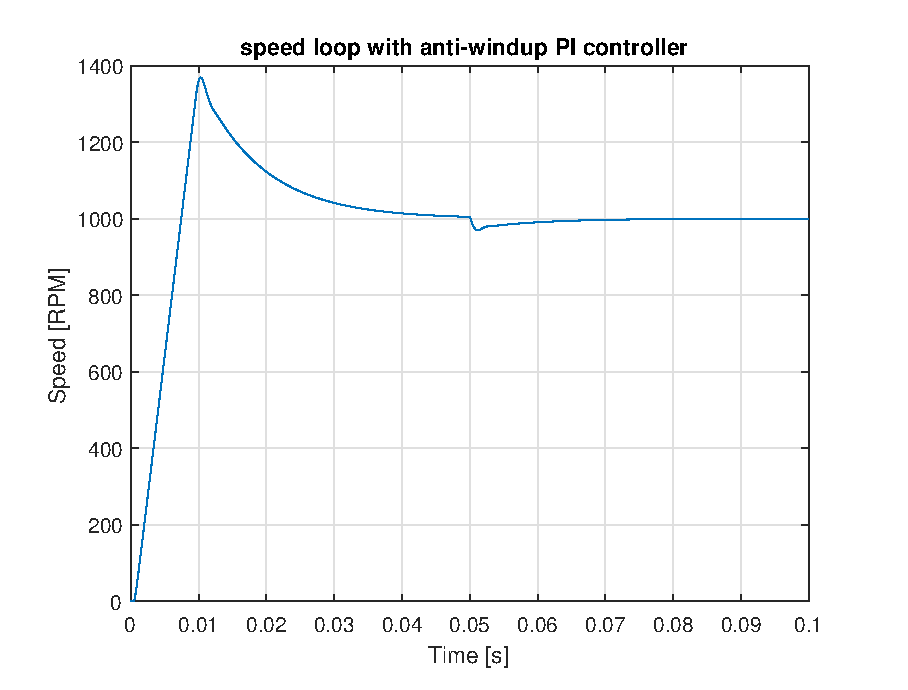
\includegraphics[height=4cm]{figs/speed_loop_classical_pi.eps}}\hspace{2em}%
	\subfloat[抗饱和PI控制器转速响应]{%
		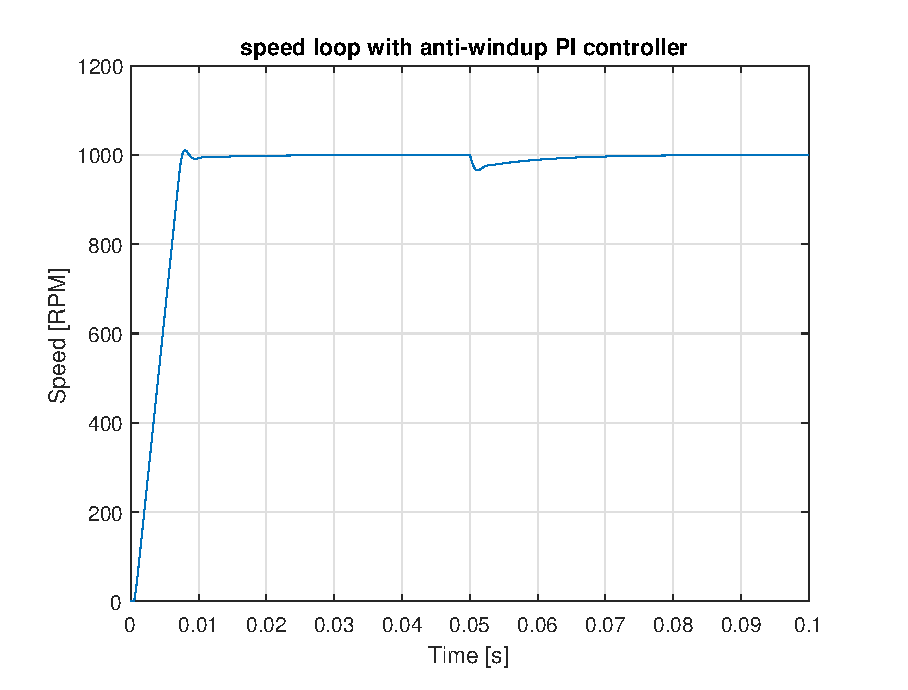
\includegraphics[height=4cm]{figs/speed_loop_antiwindup_pi.eps}}
	\caption{PI控制与抗饱和PI控制转速闭环响应}
	\label{fig:pi_speed_loop}
\end{figure}
%图\ref{fig:speed_controller_output}为转速控制时,转速闭环控制器饱和限幅之前与饱和限幅之后的输出。
%\begin{figure} [h]
%	\centering%
%	\subfloat[饱和限幅之前控制器输出]{%
%		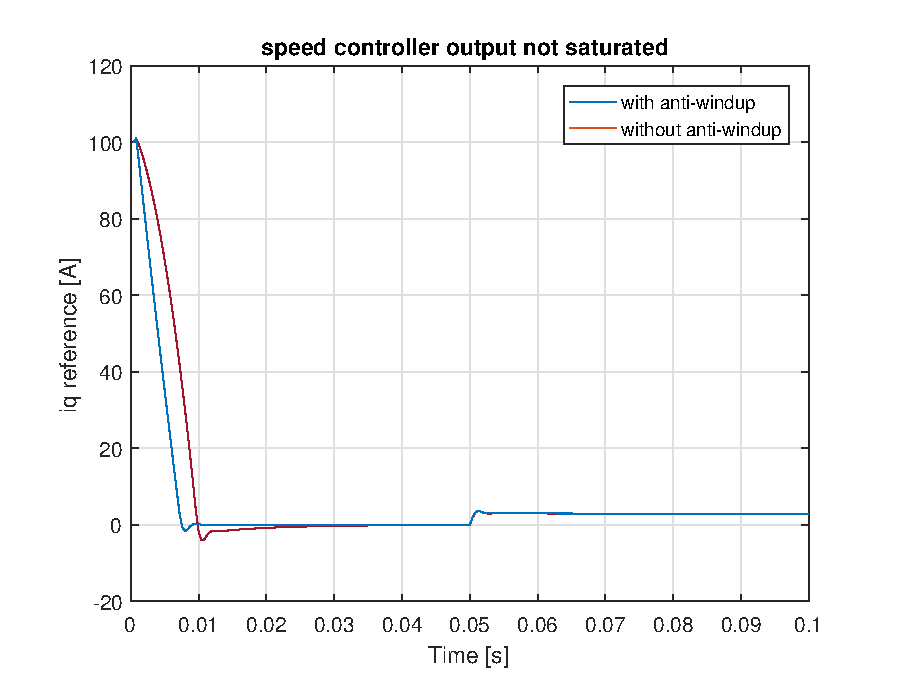
\includegraphics[height=4cm]{figs/speed_controller_output_not_saturated.eps}}\hspace{2em}%
%	\subfloat[抗饱和PI控制器转速响应]{%
%		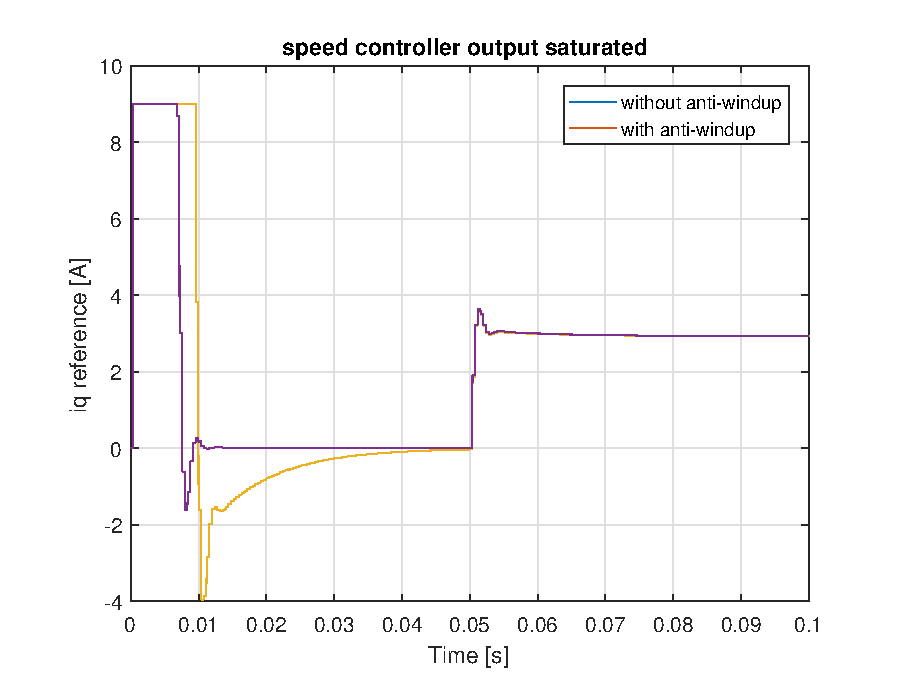
\includegraphics[height=4cm]{figs/speed_controller_output_saturated.eps}}
%	\caption{饱和限幅之后控制器输出}
%	\label{fig:speed_controller_output}
%\end{figure}

图\ref{fig:speed_controller_out_not_saturated}和图\ref{fig:speed_controller_out_saturated}分别为转速闭环控制器经饱和限幅之前与之后的输出。由该图可知,在控制器输出未饱和时,抗饱和PI与传统PI响应一样。当控制器输出饱和时,抗饱和PI控制器由于积分器中叠加了抗饱和成分,能使控制更快地退出饱和,从而减小系统超调。
\begin{figure}[H]
	\centering
	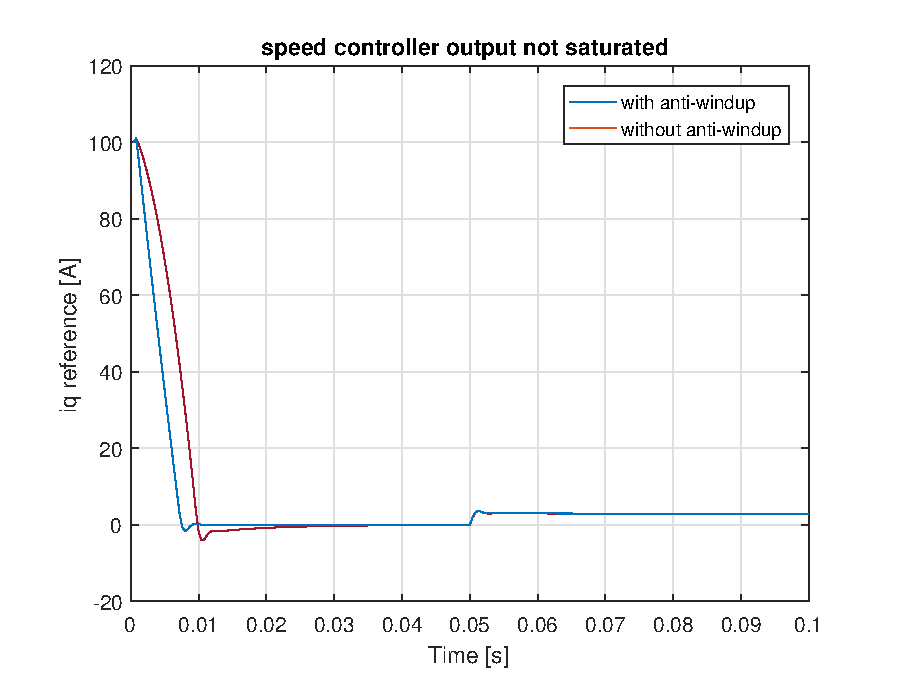
\includegraphics[width=0.7\textwidth]{figs/speed_controller_output_not_saturated.eps}
	\caption{转速控制器经饱和限幅之前的输出}
	\label{fig:speed_controller_out_not_saturated}
\end{figure}
\begin{figure}[H]
	\centering
	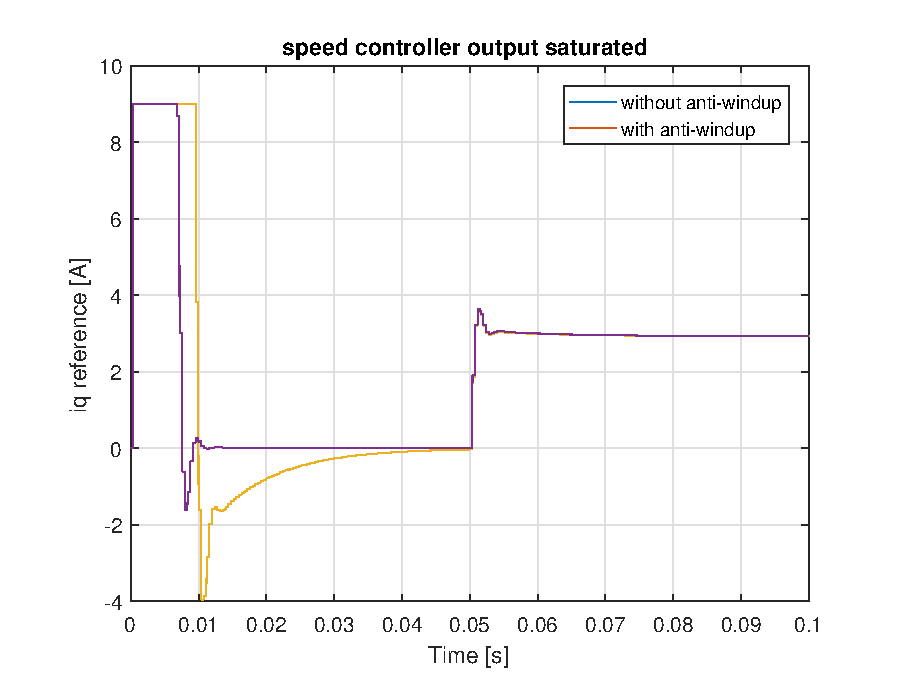
\includegraphics[width=0.7\textwidth]{figs/speed_controller_output_saturated.eps}
	\caption{转速控制器经饱和限幅之后的输出}
	\label{fig:speed_controller_out_saturated}
\end{figure}
\section{基于反电动势转子位置估算方法}
永磁同步电机矢量控制中的一个十分重要环节是获取转子位置,通常通过使用旋转编码器实现。对于高性能驱动系统,编码器十分昂贵,而且安装麻烦。无位置传感器算法利用电流电压信息以及电机参数估算转子位置,可以降低驱动成本,提高驱动系统鲁棒性。对于永磁同步电机,通常存在两种转子位置估算方法,基于反电动势法和基于高频电压注入法,本节主要介绍基于反电动位置估算方法以及应用场合。
\subsection{基本工作原理}
根据\ref{sec:model}可知,永磁同步电机在dq0参考系下的电压方程可以表示为:
\begin{equation}
\begin{gathered}
v_{q}=Ri_{q}+p\lambda_{q}+\omega_{r}\lambda_{d} \\ v_{d}=Ri_{d}+p\lambda_{d}-\omega_{r}\lambda_{q}
\end{gathered}\label{eq:1}
\end{equation}
磁链方程可表示为:
\begin{equation}
\begin{gathered}
\lambda_{q}=(L_{ls}+L_{mq})i_{q}=L_{q}i_{q}\\ \lambda_{d}=(L_{ls}+L_{md})i_{d}+\lambda_{mpm}=L_{d}i_{d}+\lambda_{mpm}
\end{gathered}\label{eq:2}
\end{equation}
将方程\ref{eq:1}和方程\ref{eq:2}改写成复数形式有:
\begin{equation}
\begin{gathered}
\bar{v}_{dq}=R\bar{i}_{dq}+j\omega_{r}(\bar{_\lambda}_{dq})\\\bar{\lambda}_{dq}=L_{d}i_{d}+\lambda_{mpm}+jL_{q}i_{q}
\end{gathered}\label{eq:3}
\end{equation}
对方程\ref{eq:3}进行dq0到$\alpha\beta$变换得到:
\begin{equation}\label{eq:vol1}
\begin{gathered}
\bar{v}_{\alpha\beta}=R\bar{i}_{\alpha\beta}+p(\bar{_\lambda}_{\alpha\beta})\\\bar{\lambda}_{\alpha\beta}=(L_{d}i_{d}+\lambda_{mpm}+jL_{q}i_{q})e^{j\theta_{r}}
\end{gathered}\label{eq:4}
\end{equation}
对方程\ref{eq:4}中的磁链变形得到:
\begin{equation}\label{eq:5}
\bar{\lambda}_{\alpha\beta}=(L_{d}i_{d}-L_{q}i_{d}+L_{q}i_{d}\\\lambda_{mpm}+jL_{q}i_{q})e^{j\theta_{r}}
\end{equation}
对方程\ref{eq:5}整理得到:
\begin{equation}\label{eq:6}
\bar{\lambda}_{\alpha\beta}=L_{q}\bar{i}_{\alpha\beta}+[(L_{d}-L_{q})i_{d}+\lambda_{mpm}]e^{j\theta_{r}}
\end{equation}
转子位置信息可由如下方程表达:
\begin{equation}\label{eq:7}
\hat{\theta_{r}}=\arctan\frac{\lambda_{\beta}-L_{q}i_{\beta}}{\lambda_{\alpha}-L_{q}i_{\alpha}}
\end{equation}    
根据方程\ref{eq:6}和\ref{eq:7},可以知道永磁同步电机转子位置信息可以由$\alpha\beta$轴磁链和电流信息得到,方程\ref{eq:6}中虽然有$i_{d}$存在,但是其只会影响包含转子位置信息的矢量的幅值,不影响其转子位置。公式\ref{eq:7}中的$\alpha\beta$磁链可以根据电机电压模型,根据公式\ref{eq:8}对反电动势积分得到。
\begin{equation}
\begin{gathered}\label{eq:8}
\lambda_{\alpha}=\int (v_{\alpha}-Ri_{\alpha}) \mathrm{d}t\\
\lambda_{\beta}=\int (v_{\beta}-Ri_{\beta}) \mathrm{d}t
\end{gathered}
\end{equation}
\subsection{积分漂移补偿\cite{drift}}
反电动势位置估算方法中求$\alpha\beta$磁链$\bar{\lambda}_{\alpha\beta}$涉及对反电动势的积分,根据公式\ref{eq:6}可知,稳态时包含转子位置的矢量$\bar{\lambda}_{\alpha\beta}-L_{q}\bar{i}_{\alpha\beta}$的轨迹应为圆心在原点的圆。但由于电流采样会存在误差偏置,即使很小的偏置在积分器作用下也会一直方法,这导致积分计算出的$\alpha\beta$磁链带有积分漂移,如图\ref{fig:dc_removal}所示,图中$\overrightarrow{\lambda}_{L}$为上述$\bar{\lambda}_{\alpha\beta}-L_{q}\bar{i}_{\alpha\beta}$矢量,积分漂移使矢量$\overrightarrow{\lambda}_{L}$的圆心偏离原点,偏移量为$DR+jDI$。
此时,用公式\ref{eq:7}计算的转子位置为矢量$\overrightarrow{\lambda}_{L}^{\prime}$的角$\theta_{\lambda L}^{\prime}$,真正转子位置的角度为矢量$\overrightarrow{\lambda}_{L}$的角$\theta_{\lambda L}$。因此需要找到圆心漂移量,进行补偿。
\begin{figure}[H]
	\centering
	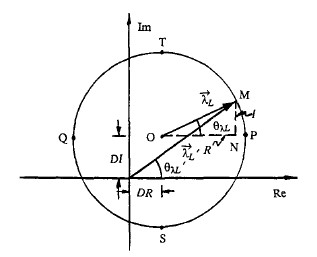
\includegraphics[width=0.7\textwidth]{figs/dc_removal.jpg}
	\caption{带积分漂移的磁链轨迹}
	\label{fig:dc_removal}
\end{figure}
根据图中4个点$P,Q,T,S$将带漂移的矢量$\overrightarrow{\lambda}_{L}$将漂移量求出,这四个点是磁链矢量轨迹圆最边缘的四点。
\begin{equation}
DR+jDI=\frac{\lambda_{LR(max)}^{\prime}+\lambda_{LR(min)}^{\prime}}{2}+j\left(\frac{\lambda_{LI(max)}^{\prime}+\lambda_{LI(min)}^{\prime}}{2} \right)
\end{equation}
其中$\lambda_{LR(max)}^{\prime}$和$\lambda_{LI(max)}^{\prime}$分别为矢量$\overrightarrow{\lambda_{L}^{\prime}}$的实部和虚部。
找出积分漂移之后,真正转子位置角度根据公式\ref{eq:EMF_position}计算。
\begin{equation}\label{eq:EMF_position}
\theta_{\lambda L}=\arctan{\left(\frac{\lambda_{LI}^{\prime}-DI}{\lambda_{LR}^{\prime}-DR}\right)}
\end{equation}
\subsection{应用场合以及影响因素}
反电动势位置估算方法需要对反电动势积分,当电机转速较低时,反电动势的值很小,此时估算不可靠。因此一般,无位置传感器反电动势位置估算方法用在中高速应用场合,比如说风机、泵等装置中。先将电机启动旋转至一定速度,再使用反电动势位置估算。对于启动动态控制性能要求不高的且工作在中高速的场合可以使用开环的方法将电机加速到一定速度,再切换到基于反电动势位置估算矢量控制\cite{wang2012simple}。对于启动动态性能要求较高的场合,在启动阶段可使用基于高频电压注入矢量控制,当电机加速到一定速度时,切换基于反电动位置估算的方法\cite{1348530}。

本文所描述的反电动势位置估算忽略了电机参数变化的影响,电机电感实际上会随着dq轴电流变化而改变\cite{lu2013artificial},电机绕组电阻值会随着温度的改变而改变,这些参数改变对反电动势位置估算方法性能的影响,参数变化时估算算法怎么设计都有待进一步研究。
\section{转子初始位置确定}
永磁同步电机FOC控制需要使用转子位置信息用来进行坐标变换,FOC控制启动前需要确定转子位置。可以使用绝对式编码器来解决这一问题,但是绝对式编码器价格昂贵。对于使用增量编码器或者无位置传感器的永磁同步电机矢量控制器来说,若确定转子初始位置时需保证电机不能旋转,则需要采用基于高频电压注入等方法检测初始位置\cite{__2013,bolognani_sensorless_1999,__2011-1,__2011}。
本文中确定转子位置时,允许电机旋转,此时使用一种简单的方法即可确定转子位置。在启动FOC控制之前,给定$\alpha$轴电压为一个比较小的固定值,$\beta$电压为0。此时将在$\alpha$轴方向产生固定磁场,该磁场与转子永磁磁场相互作用,使转子旋转至N级即d轴与定子a相磁轴重合,此时转子位置$\theta_{r}=0$,这样之后才可以开始矢量控制。
\section{本章小结}
本章主要介绍了永磁同步电机矢量控制思想,详细研究了矢量控制中电流内环、速度外环参数调节方法、基于反电动势的位置估算以及位置估算算法中漂移补偿方法和一种简单矢量控制启动前将电机转子位置置零的方法。